\documentclass[9pt]{beamer}
\usetheme{Boadilla}
\usepackage[utf8]{inputenc}
\usepackage{amsmath}
\usepackage{amsfonts}
\usepackage{amssymb}
\usepackage{graphicx}
\usepackage{xcolor}
\author{Adriano Del Vincio}
\usepackage[output-decimal-marker={.}]{siunitx}
\title[Alpha 2]{Toy Model For Hyperfine Measurement}

\setbeamercolor{block title}{fg=white, bg = cyan }
\author[Adriano, Germano, Simone]{Adriano Del Vincio, Germano Bonomi,\\ Simone Stracka}
%\setbeamercovered{transparent} 
%\setbeamertemplate{navigation symbols}{} 
\logo{
\includegraphics[width = 0.125\textwidth]{../../../logo/ALPHA_Logo.jpg}}
\newcommand{\nologo}{\setbeamertemplate{logo}{}}
\institute[]{University of Brescia, INFN Pisa} 
\titlegraphic{
\begin{figure}
\hspace{1.cm}

\includegraphics[width = 0.12\textwidth ]{../../../logo/logounibs.png}
%\hspace{1cm}

\includegraphics[width = 0.25\textwidth ]{../../../logo/1_Pisa_LOGO_SIGLA.pdf}
\end{figure}
} 
\beamertemplatenavigationsymbolsempty
\begin{document}

\begin{frame}
\titlepage
\end{frame}

%\begin{frame}
%\tableofcontents
%\end{frame}

\begin{frame}{Scheme of the Simulation}
Scheme of the Monte Carlo Toy for generating the events

\begin{figure}
\centering
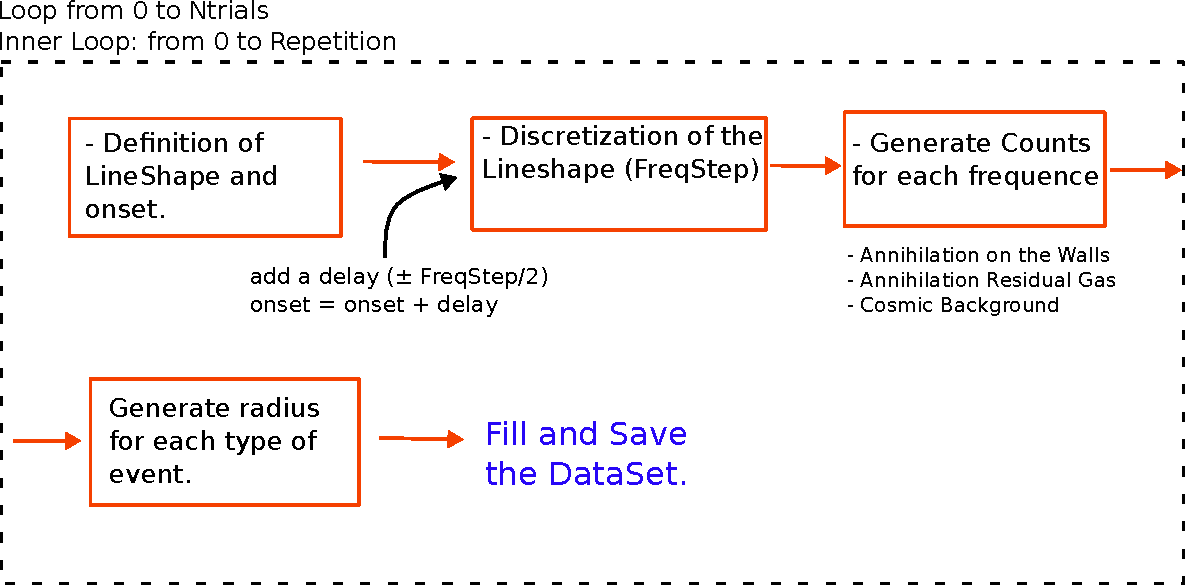
\includegraphics[width = 0.95\textwidth]{SimulationScheme.pdf}
\end{figure}

\begin{center}
In this simulation, the data are created and analyzed using\newline \textit{RDataFrame} framework.
\end{center}

\end{frame}

\begin{frame}{A brief introduction about the Monte Carlo}

We have developed a Monte Carlo Toy that produces two \texttt{.root} dataset files. The variables are columns of values that are shown in the figure below:
\begin{figure}[hbtp]
 \centering
 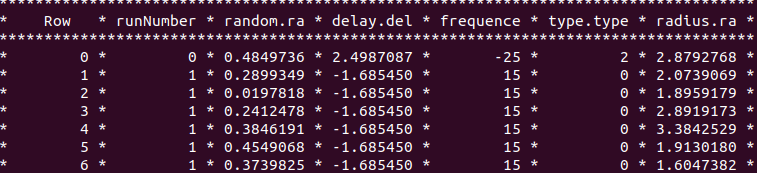
\includegraphics[width = 0.75\textwidth]{DatasetContent.png}
 \caption{ Structure of the dataset.}
 \end{figure}

\begin{itemize}
\item \textit{runNumber}: identifies which run the event belong to (from $0$ to $Repetition -1$) 
\item \textit{random}: values uniform distributed from $0$ to $1$, can be used to randomize the selection or for sub-sampling in the data
\item \textit{delay}: store the onset delay
\item \textit{frequence}: the frequency of the event
\item \textit{type}: type of the event: 0 annihilation on the walls, 1 residual gas annihilation, 2 cosmic event
\item \textit{radius}: radius of the annihilation vertex.
\end{itemize}

\end{frame}

\begin{frame}{A brief introduction about the Monte Carlo}

The Annihilation on the walls are generated as function of the frequency, using the two line-shapes of the transitions (c $\rightarrow$ b) and (d $\rightarrow$ a). The Annihilation on the residual gas and the cosmic background are generated uniformly on the frequency spectrum. All the parameters of the simulation are loaded from the \texttt{ToyConfiguration.txt} file. The parameters are chosen to reproduce the runs 4b.

\begin{figure}[hbtp]
\centering
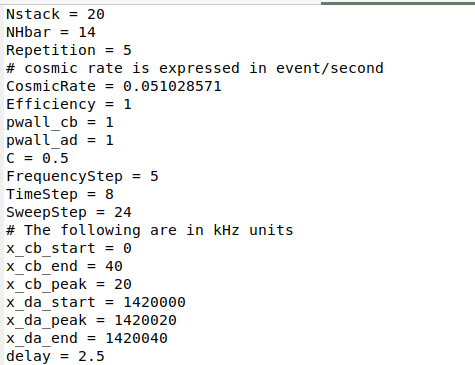
\includegraphics[width = 0.5\textwidth]{MontecarloParams.png}
\caption{ Parameters of the Toy.}
\end{figure}
\end{frame}

\begin{frame}{Triangular Line-shape Pdfs}

For this first use of the toy, we have chosen simple line-shapes, triangular with a symmetric rise and fall.

\begin{figure}
\centering
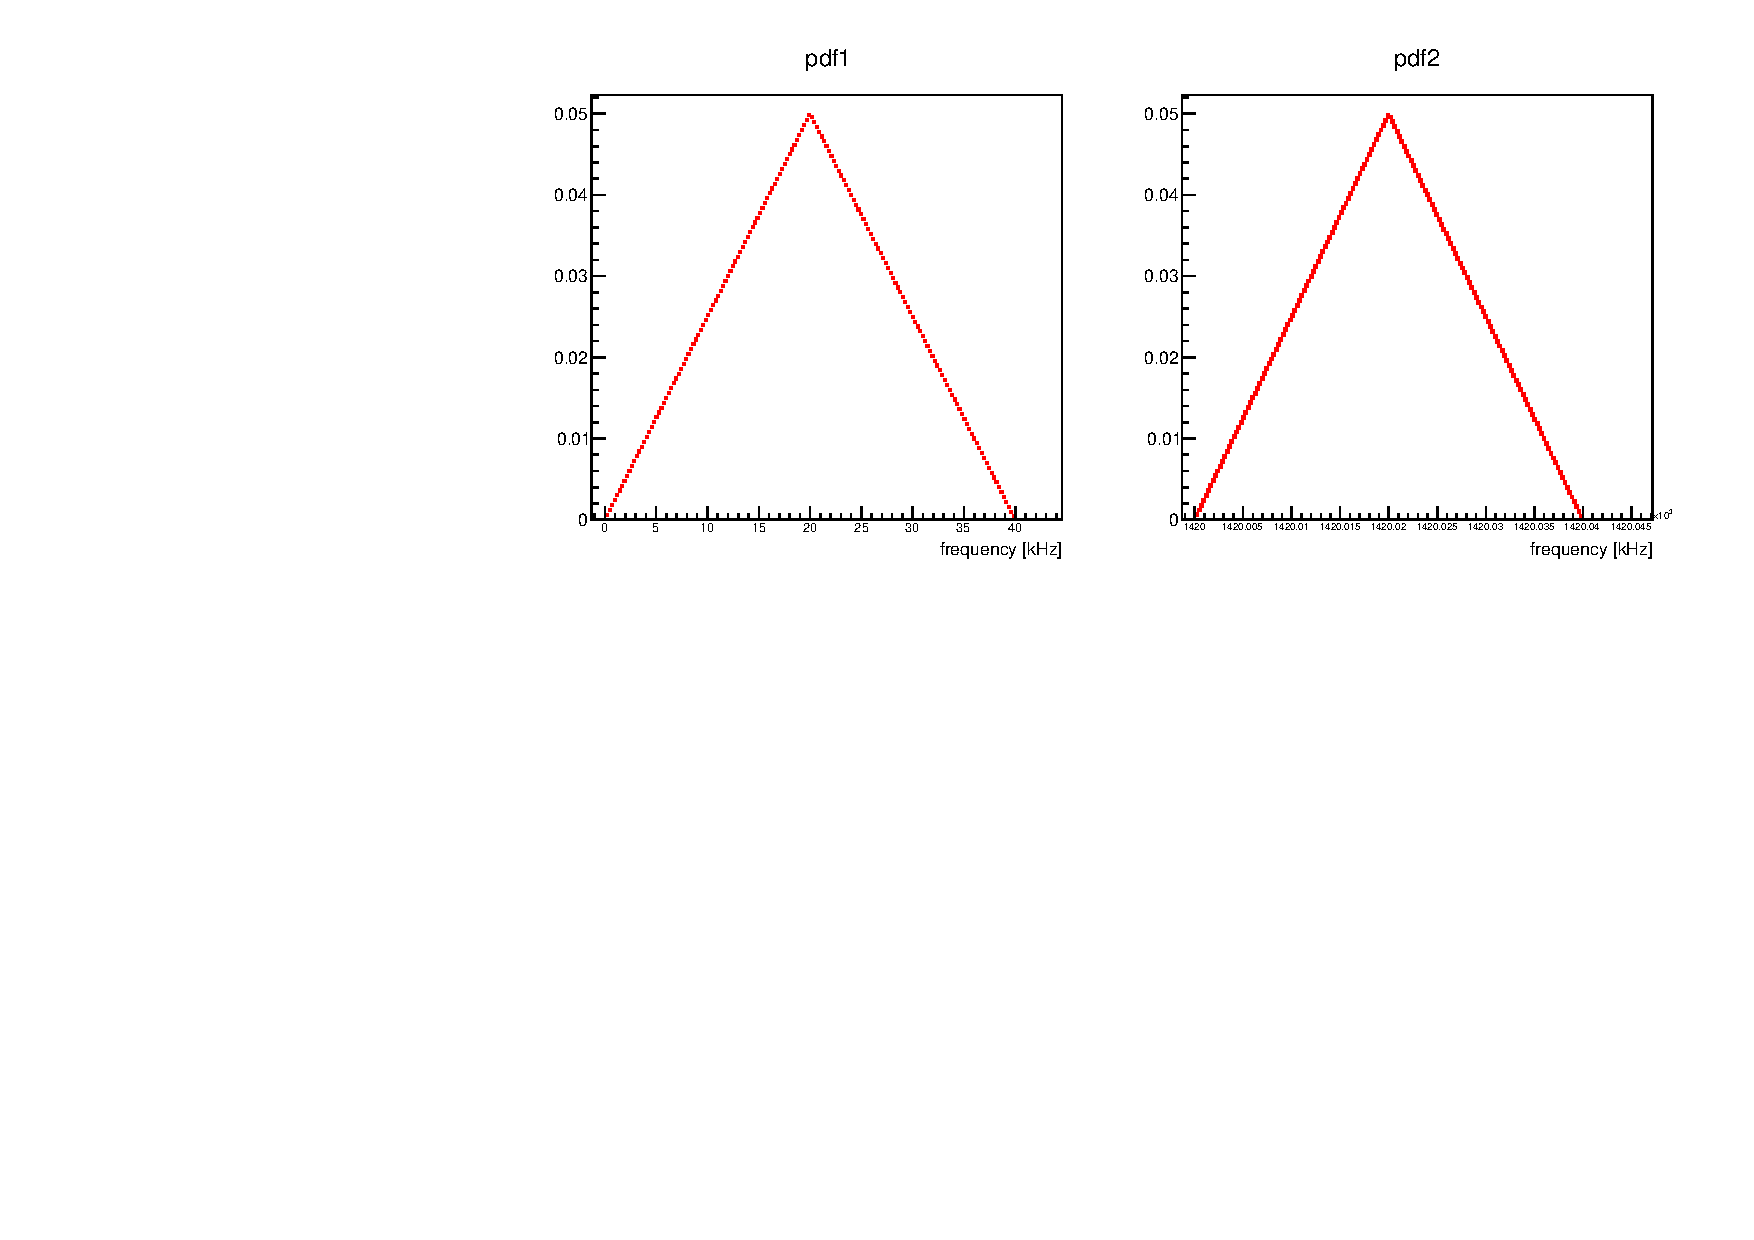
\includegraphics[width = \textwidth]{../Plot/Pdf1Pdf2.pdf}
\end{figure}

\end{frame}

\begin{frame}{Triangular Line-shapes Simulation}

We sample at the given frequency step of $\SI{5}{ \kilo \hertz}$ the Pdfs, to simulate the experimental line-shapes. We applied the onset finding algorithm to this distribution.
 
\begin{figure}
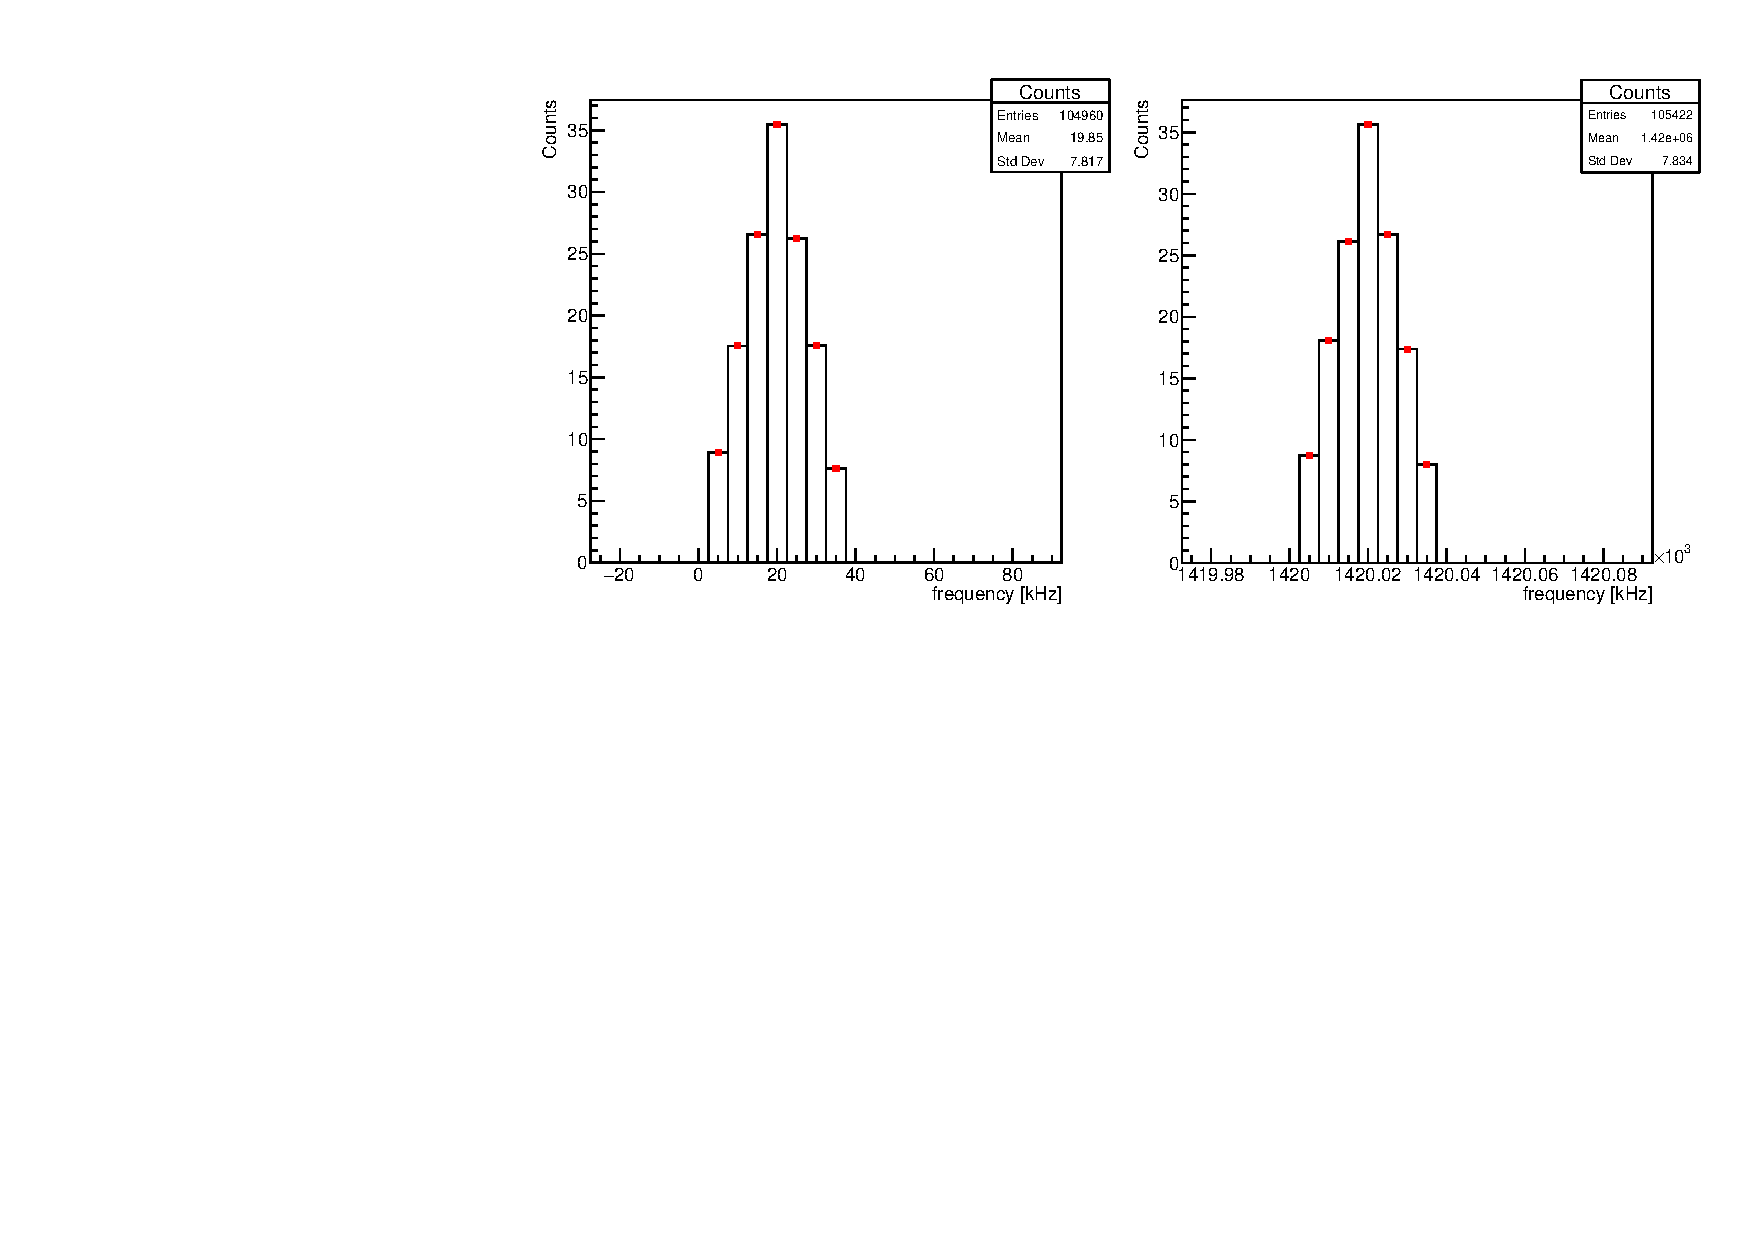
\includegraphics[width = \textwidth]{TriangleLineShape.pdf}
\end{figure}

The onset is fixed ad $f = \SI{0}{\kilo \hertz}$. In this sample the cosmic background is\newline set to zero.

\end{frame}

\begin{frame}{A simple Onset finding Algorithm}

The first algorithm that is tested is quite simple: {\color{red}{ \textbf{the onset is identified by the first bin with a content over a given threshold}} ($> N\mu_{cosmic}$)} \footnote{Where the $\mu_{cosmic}$ is computed from the Poisson distribution of the cosmic counts expected per bin.}

Before showing the plot with the simulated data, it is useful to remind how this algorithm deals with the frequency step:

\begin{figure}
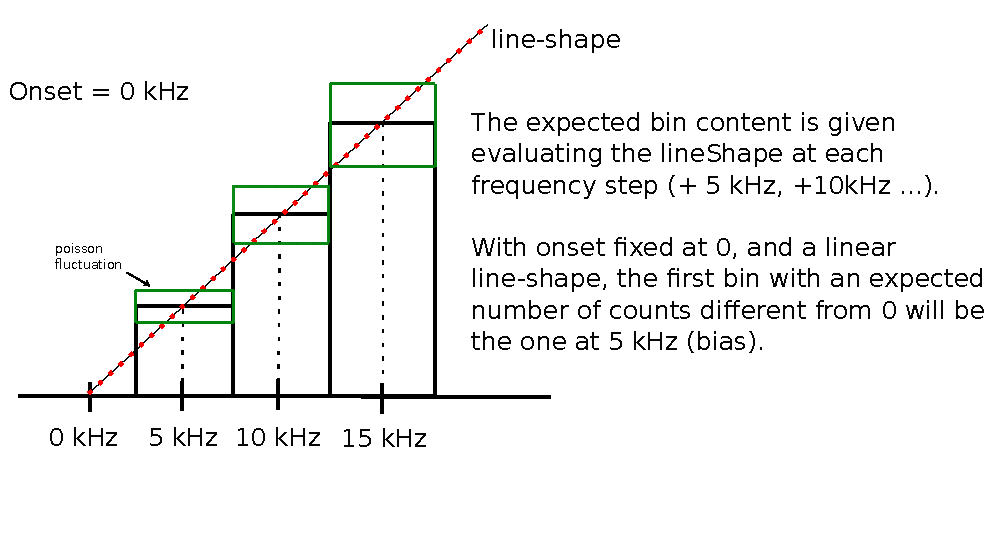
\includegraphics[width = 0.9\textwidth]{ExplainingAlgorithm1.pdf}
\end{figure}
\end{frame}

\begin{frame}{Consistency Check 1}

We have tested the algorithm with a dataset without cosmic background and delay fixed to zero. The algorithm identifies the onset at frequency $\SI{5}{\kilo \hertz}$.

\begin{figure}
\includegraphics[width = 0.9\textwidth]{../Plot/OnsetResult.pdf}
\end{figure} 
\end{frame}

\begin{frame}{Consistency Check 2}

We have tested the algorithm with a dataset without cosmic background. The delay is uniform distributed in $\SI{-2.5}{\kilo \hertz}$ and $\SI{+2.5}{\kilo \hertz}$.

\begin{figure}
\includegraphics[width = 0.9\textwidth]{../Plot/OnsetResult7.pdf}
\end{figure} 
\end{frame}

\begin{frame}{Consistency Check 2}

With the delay, two bins ( $frequency = \SI{0}{\kilo \hertz}$ and $frequency = \SI{5}{\kilo \hertz}$) are populated.  
\begin{figure}
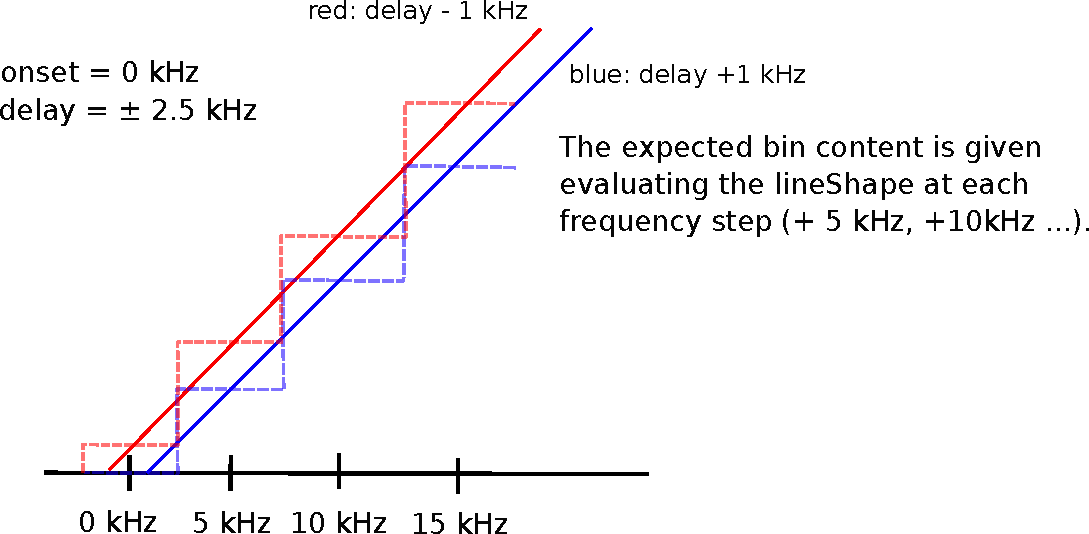
\includegraphics[width = 0.9\textwidth]{ExplainingAlgorithm2.pdf}
\end{figure}
\end{frame}

\begin{frame}{algorithm test: threshold $ > 3 \mu_{cosmic}$}

In this case, we have applied the algorithm to simulated data with cosmic background (using a rate of $0.051 \frac{event}{s}$, from passcut1). Each bin has an expected cosmic background of $dwelltime \cdot rate = 0.408$.
The delay is uniform distributed in $\SI{-2.5}{\kilo \hertz}$ and $\SI{+2.5}{\kilo \hertz}$. 
\begin{figure}
\includegraphics[width = 0.9\textwidth]{../Plot/OnsetResult11.pdf}
\end{figure}
\end{frame}

\begin{frame}{algorithm test: threshold $ > 5 \mu_{cosmic}$}

In this case, we have applied the algorithm to simulated data with cosmic background (using a rate of $0.051 \frac{event}{s}$, from passcut1). Each bin has an expected cosmic content of $dwelltime \cdot rate = 0.408$.
The delay is uniform distributed in $\SI{-2.5}{\kilo \hertz}$ and $\SI{+2.5}{\kilo \hertz}$. 
\begin{figure}
\includegraphics[width = 0.9\textwidth]{../Plot/OnsetResult12.pdf}
\end{figure}

\end{frame}


\begin{frame}{algorithm test: threshold $ > 8 \mu_{cosmic}$}

In this case, we have applied the algorithm to simulated data with cosmic background (using a rate of $0.051 \frac{event}{s}$, from passcut1). Each bin has an expected cosmic content of $dwelltime \cdot rate = 0.408$.
The delay is uniform distributed in $\SI{-2.5}{\kilo \hertz}$ and $\SI{+2.5}{\kilo \hertz}$. 
\begin{figure}
\includegraphics[width = 0.9\textwidth]{../Plot/OnsetResult15.pdf}
\end{figure}

\end{frame}

\begin{frame}{Next step}
\begin{itemize}
\item different line-shapes (e.g. quadratic rise, etc.)
\item different onset-finding algorithm
\item simulation of repetition/runs with Bfield drift.
\end{itemize}
\end{frame}

\begin{frame}{ Improvements of the week (24/11/30 - 24/12/07)}
\begin{itemize}
\item Implemented the onset-finding algorithm of 2017 ($first > 0 , second > 1$)
\item Simulation with a lineShape following the \texttt{ run 69373 } (lineShape with high statistics).
\item Implementation and test of different onset finding algorithms.
\end{itemize}
\end{frame}

\begin{frame}{Fit to the data of run 69373}

The lineShape is fitted using a Cruijff function, which takes into account the asymmetry of the left-right tails, ($model = N \cdot exp(  \frac{-(x - x_{0})^2}{2\sigma_{0,1} + k_{0,1}(x - x_{0})^{2}})$) 

\begin{figure}[hbtp]
\centering
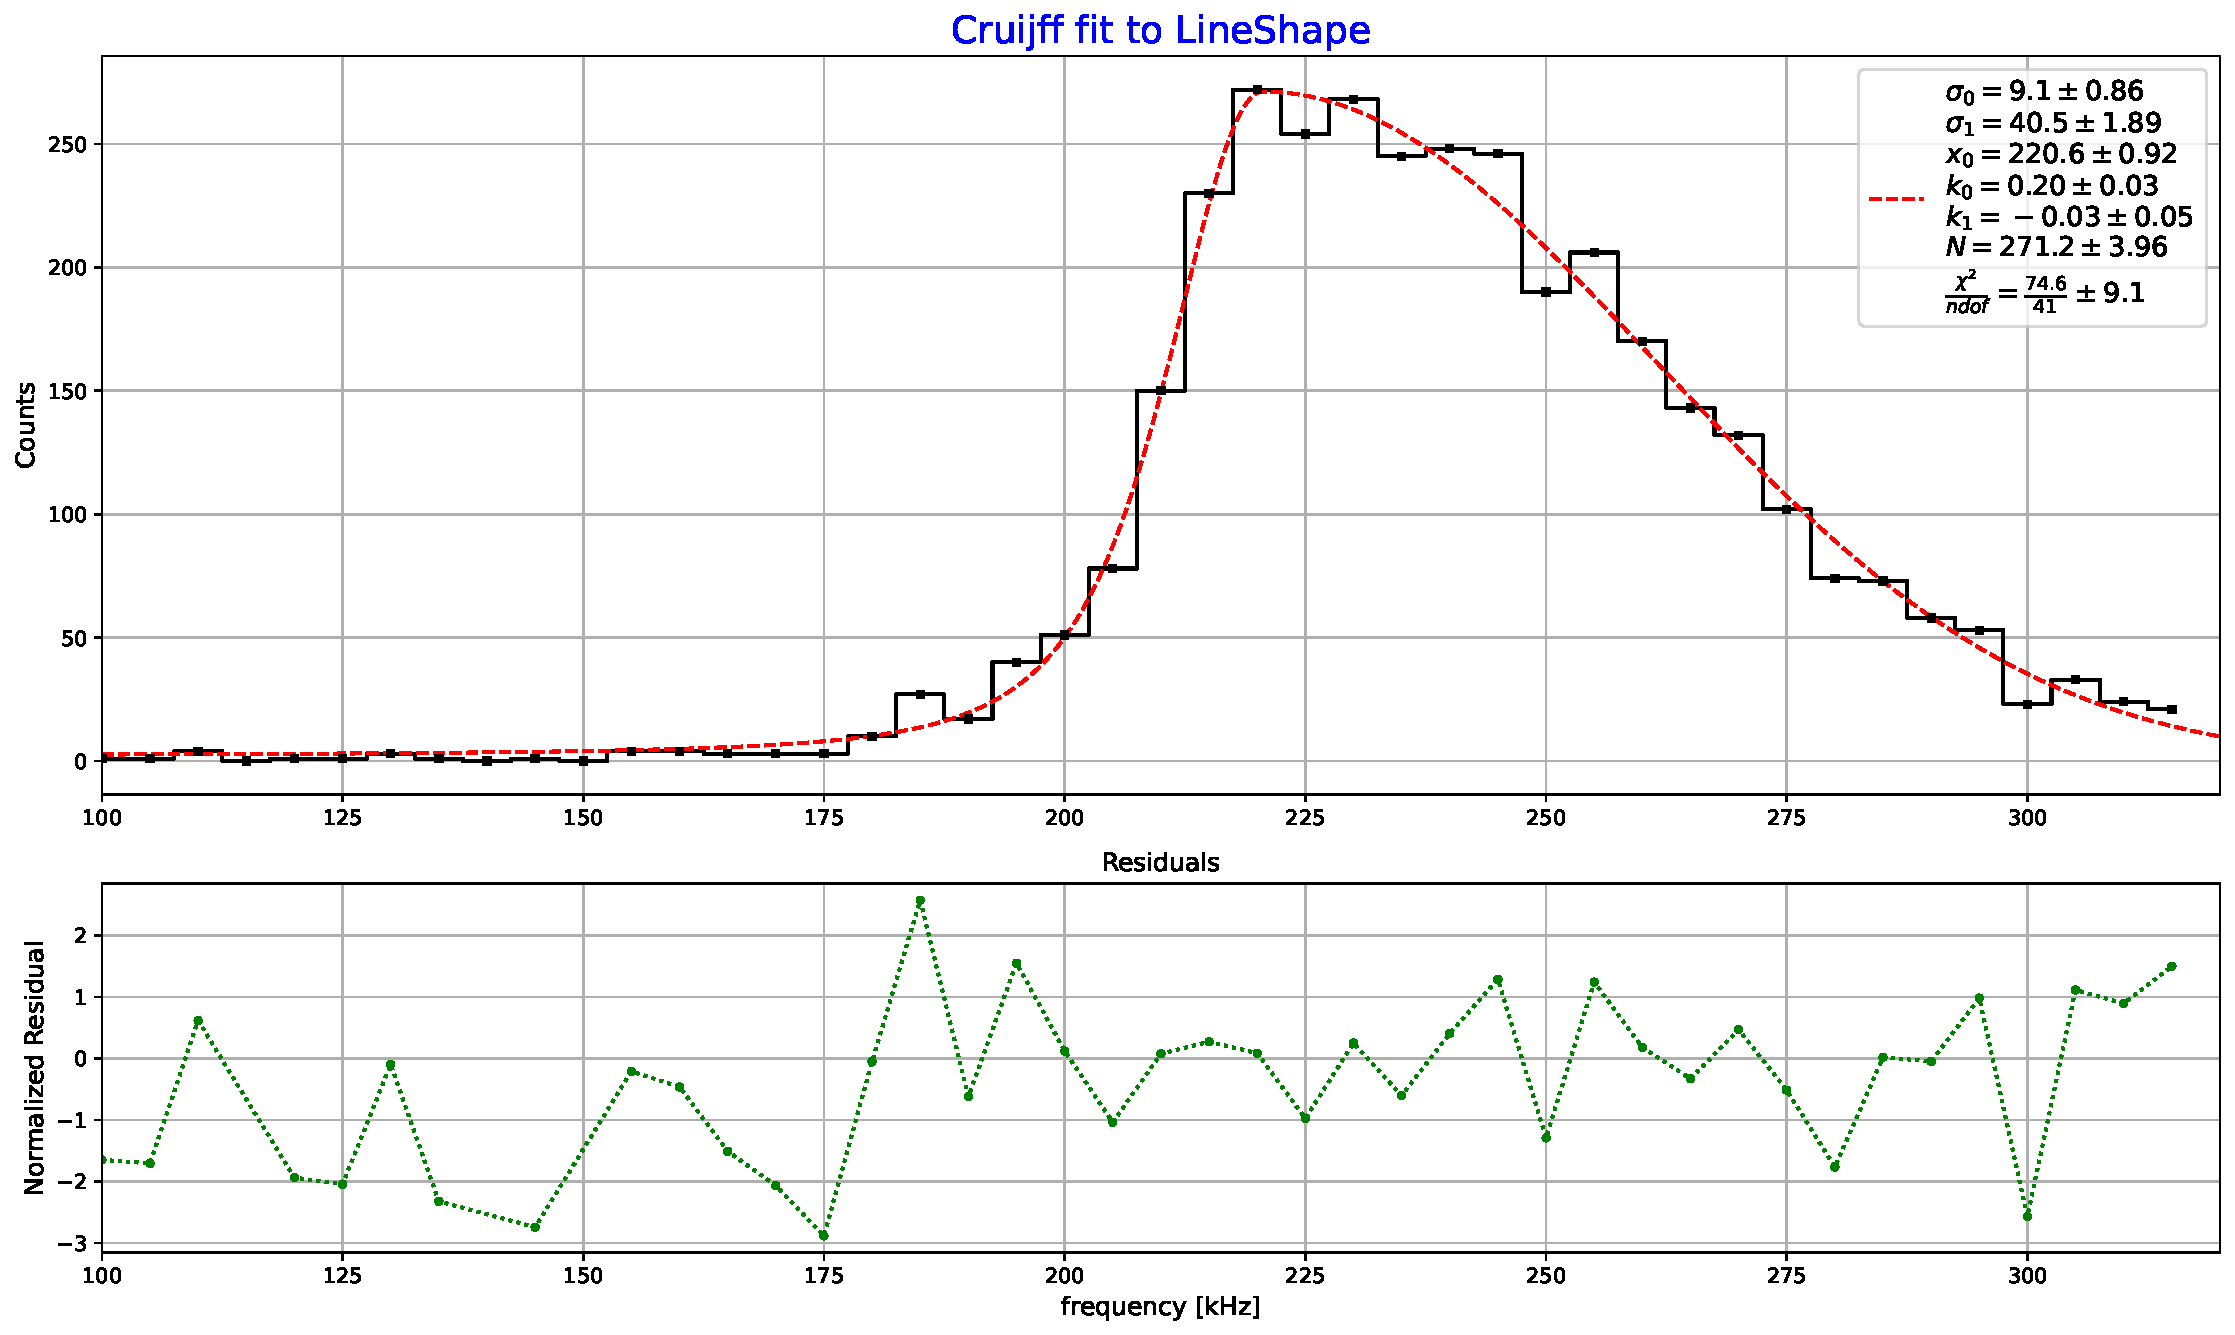
\includegraphics[width = 0.8\textwidth ]{../Plot/FitToLineShape.pdf}
\caption{On top plot, the black line represents data and the red line the fit with the\newline Cruijff function.}
\end{figure}
\end{frame}

\begin{frame}
\begin{figure}[hbtp]
\centering
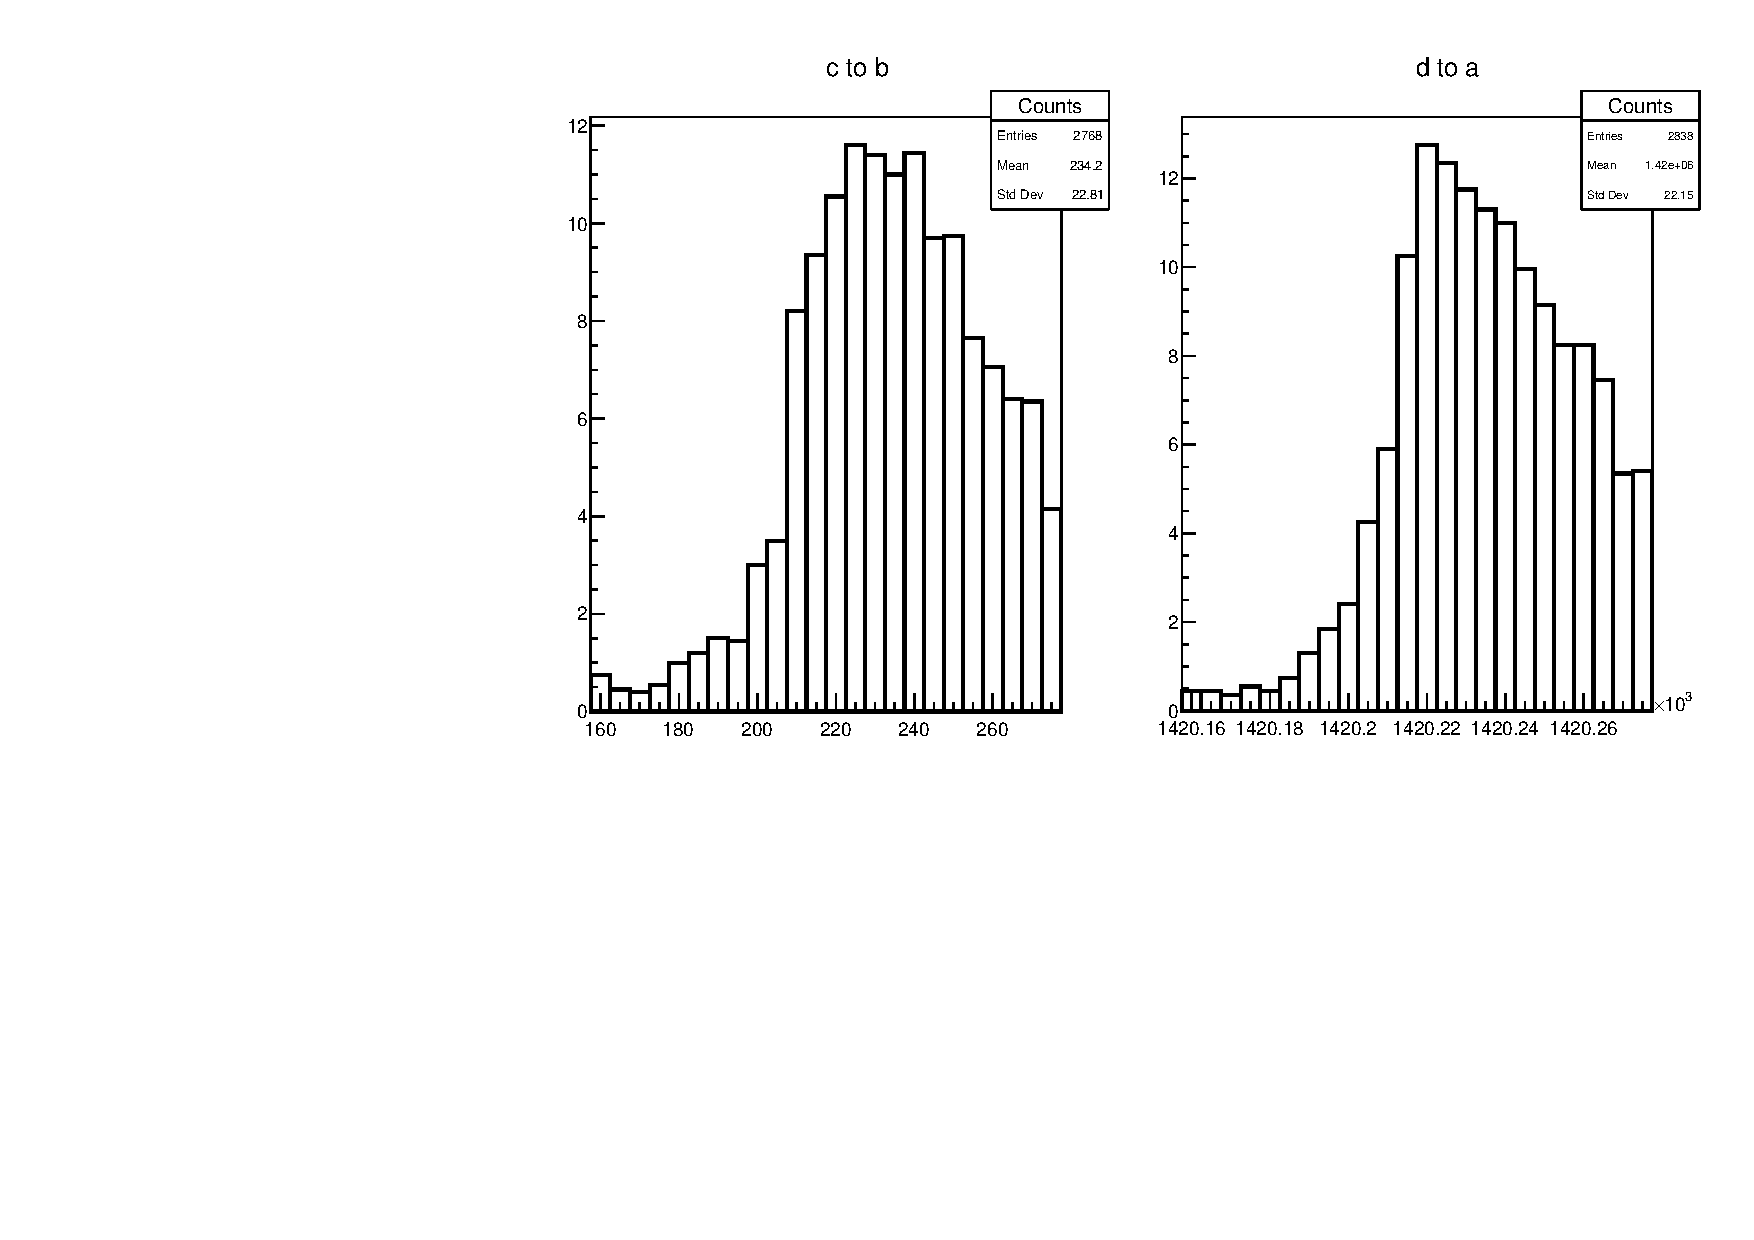
\includegraphics[width = \textwidth]{../Plot/LineshapeSampled.pdf}
\caption{ Histogram of the generated lineshape for 20 run. The Lineshape is scaled by a\newline factor of 20.}
\end{figure}
\end{frame}

\nologo{
\begin{frame}{test 2017 algorithm}

The algorithm is tested for $N_{trial} = 1000$. In this first scenario the cosmic events are removed from the data.

\begin{figure}[hbtp]
\centering
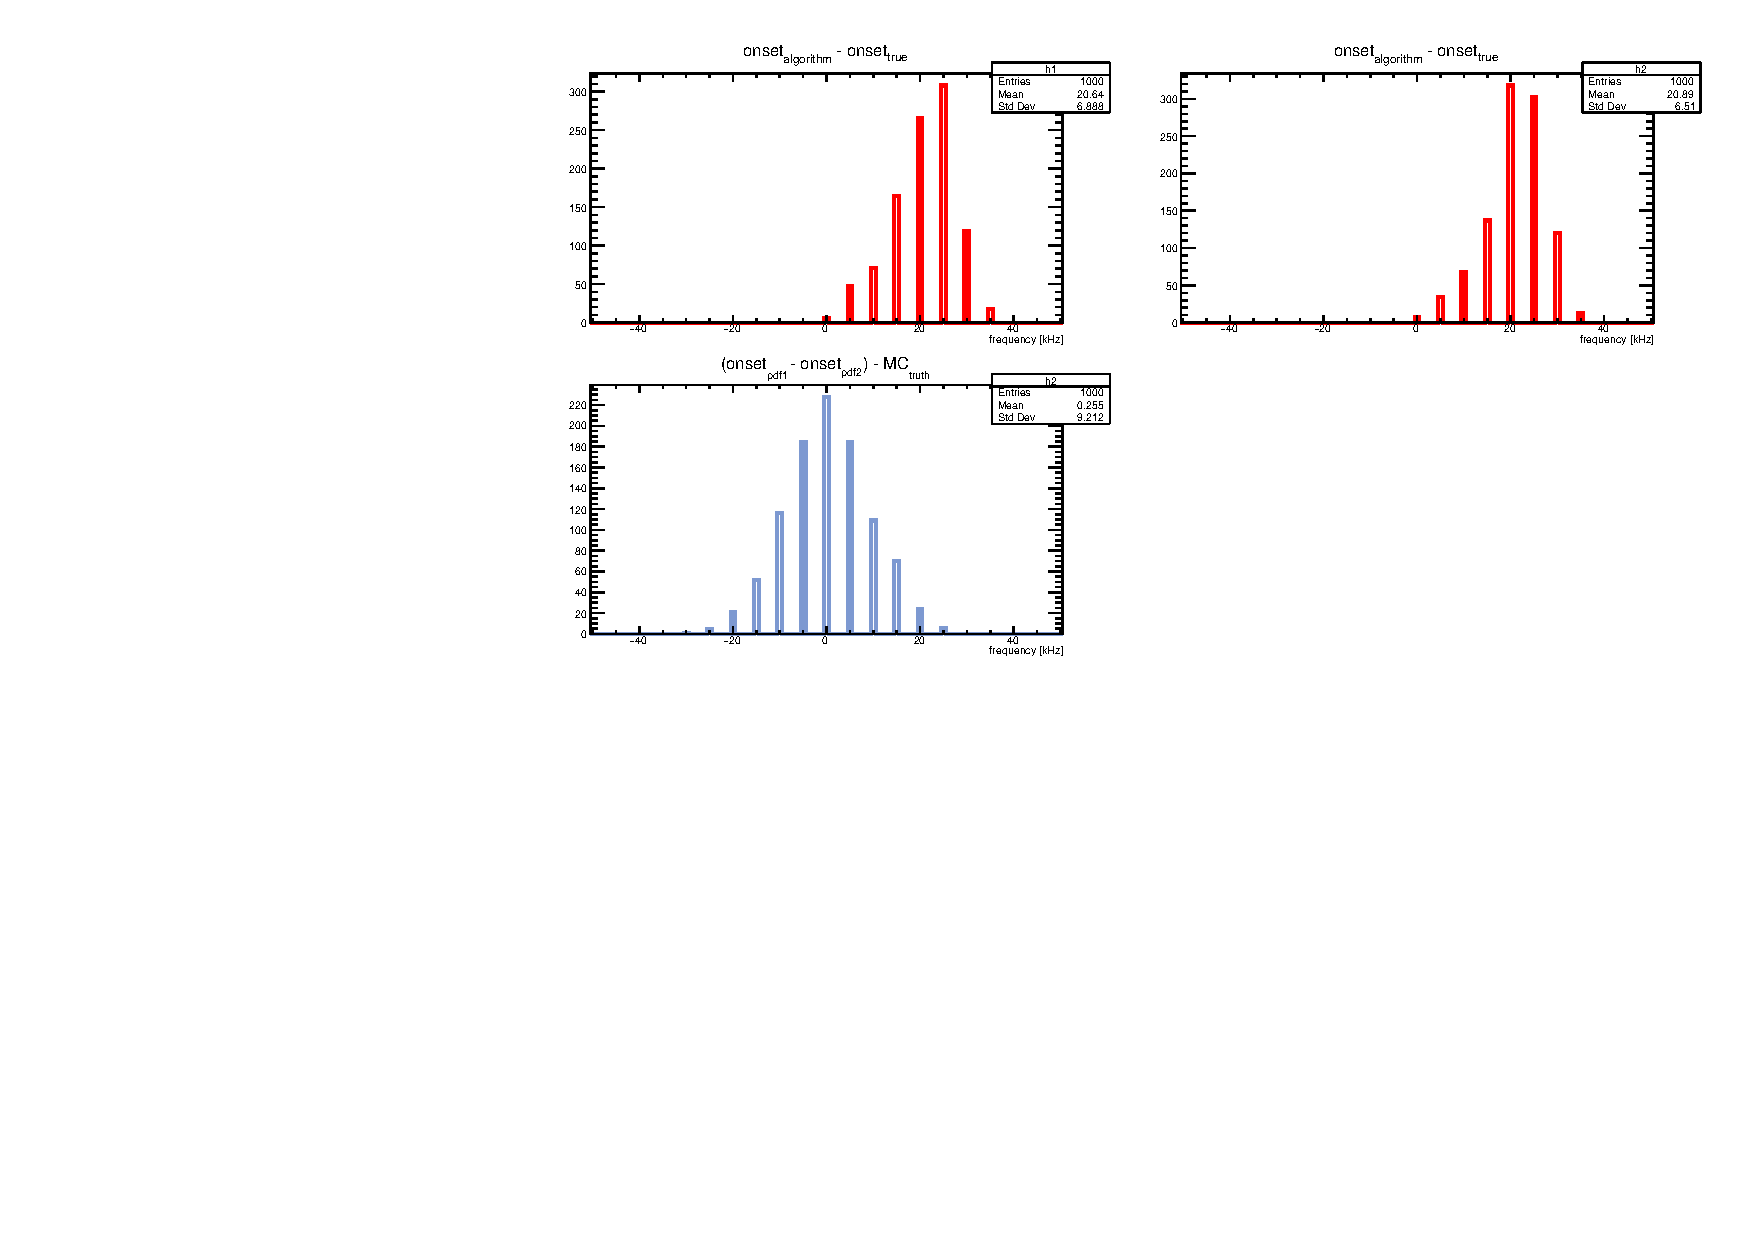
\includegraphics[width = 1\textwidth]{../Plot/2017_foward(cosmic=0).pdf}
\end{figure}
\end{frame}
}

\nologo{
\begin{frame}{test 2017 algorithm}

The algorithm is tested for $N_{trial} = 1000$. The cosmic background is fixed to $0.41$ events per frequence.

\begin{figure}[hbtp]
\centering
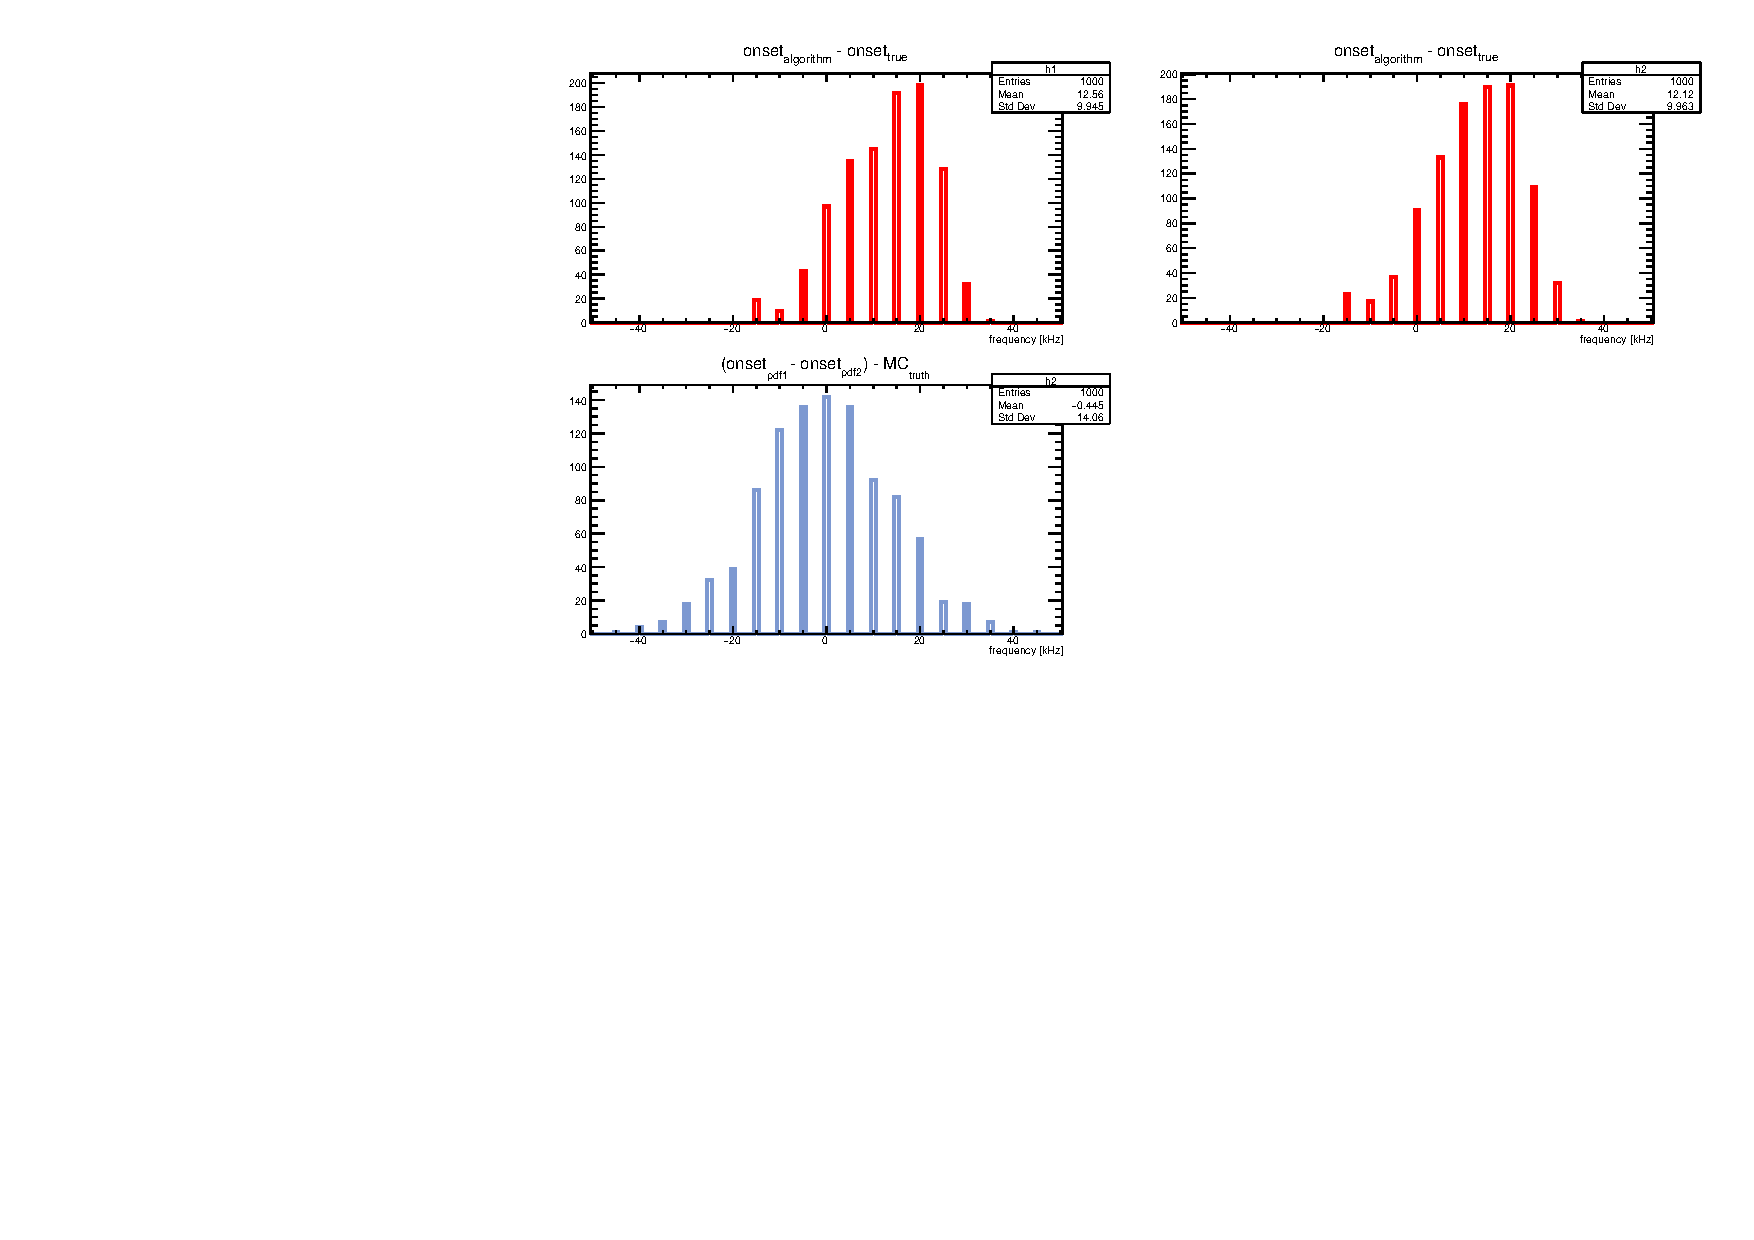
\includegraphics[width = 1\textwidth]{../Plot/2017_foward.pdf}
\end{figure}
\end{frame}
}

\nologo{
\begin{frame}{test 2017 algorithm (reversed)}

The algorithm is tested for $N_{trial} = 1000$. In this scenario the cosmic background is removed.

\begin{figure}[hbtp]
\centering
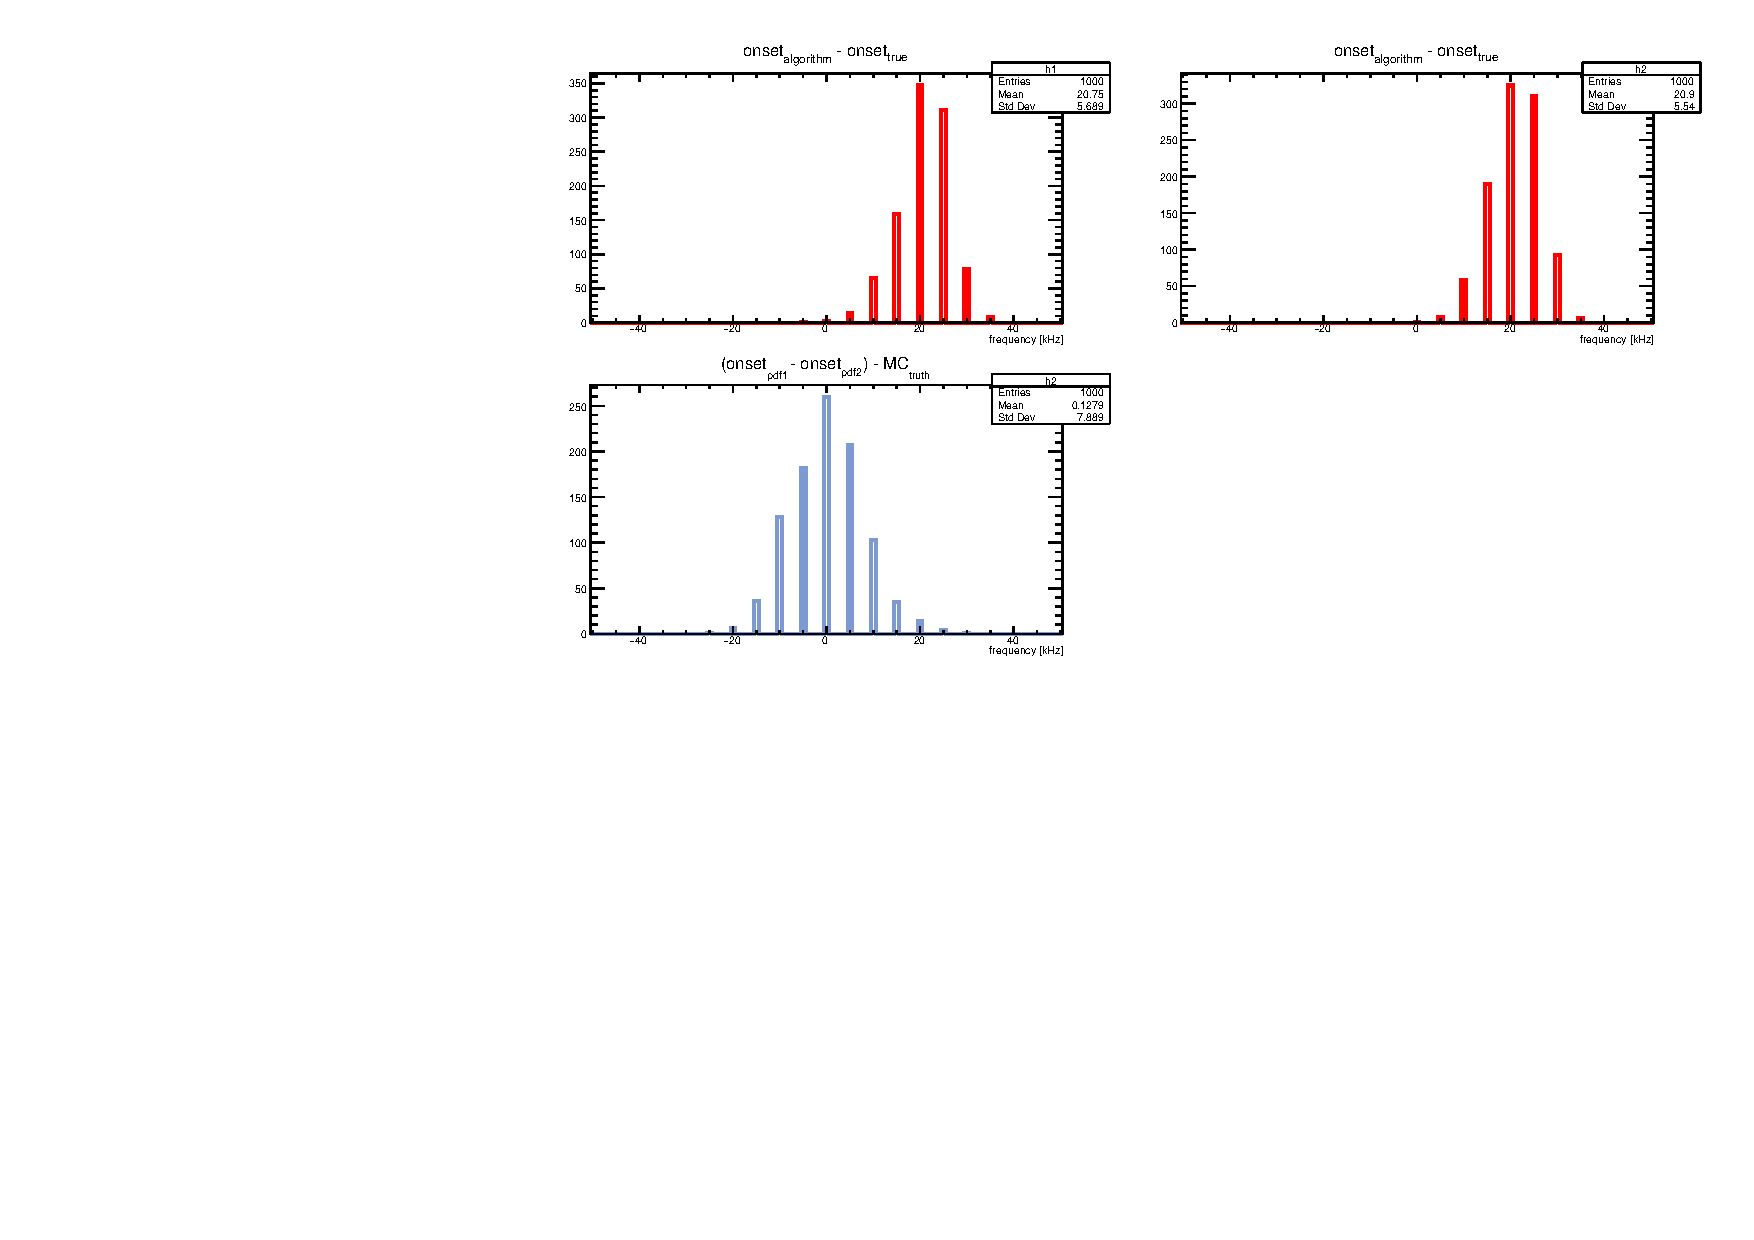
\includegraphics[width = 1\textwidth]{../Plot/2017_reversed(cosmic=0).pdf}
\end{figure}
\end{frame}
}

\nologo{
\begin{frame}{test 2017 algorithm (reversed)}

The algorithm is tested for $N_{trial} = 1000$. The cosmic background is fixed to $0.41$ events per frequence. 

\begin{figure}[hbtp]
\centering
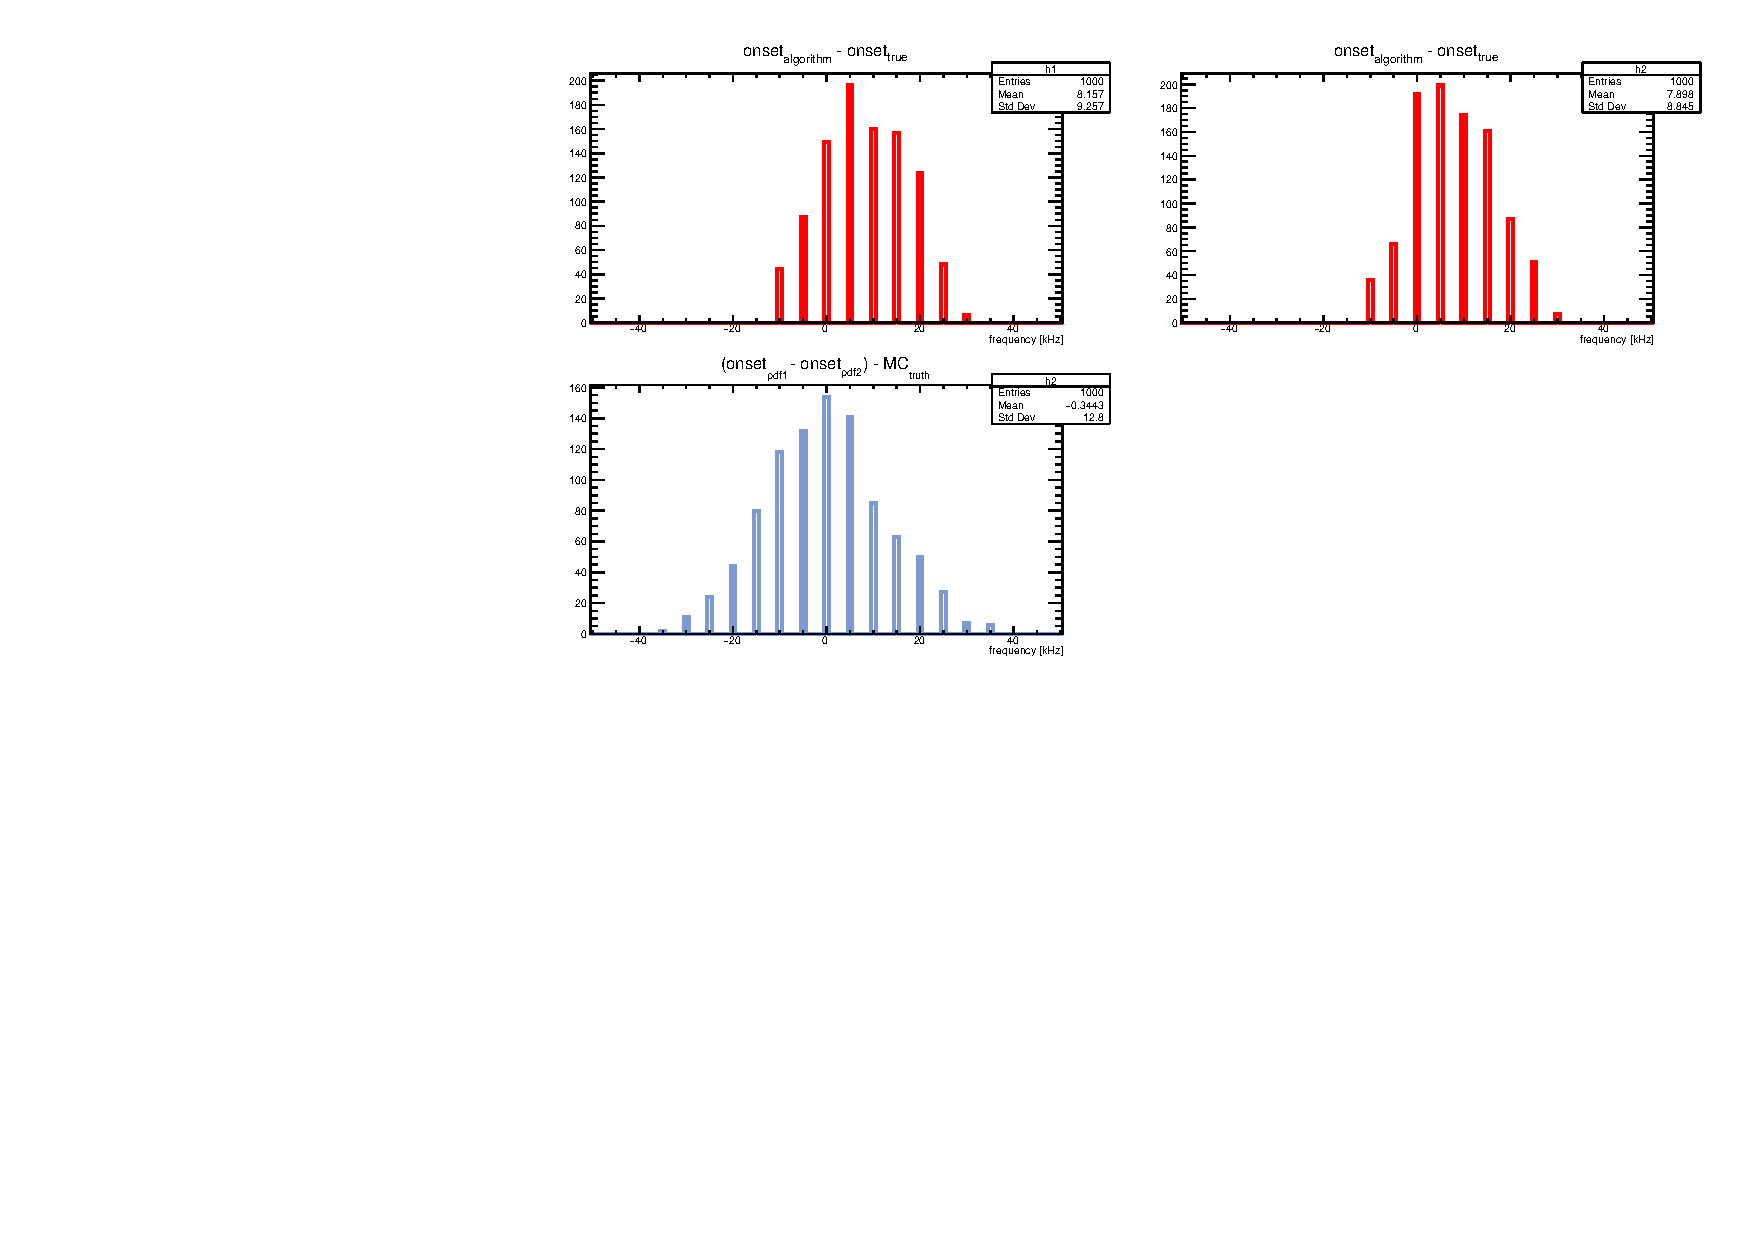
\includegraphics[width = 1\textwidth]{../Plot/2017_reversed.pdf}
\end{figure}
\end{frame}
}

\end{document}